\documentclass{article}
\usepackage{hyperref}
\usepackage{listings}
\usepackage{color}
\usepackage{xcolor}
\usepackage{geometry}
\usepackage{graphicx}
\usepackage{amsmath}
\usepackage{caption}
\usepackage{subcaption}
\usepackage[capitalise]{cleveref}
\usepackage{wrapfig}
\usepackage{amssymb}

\geometry{margin=1in}
\pdfminorversion=6

\newcommand\TODO[1]{\textcolor{red}{TODO: #1}}

\newcommand\header[2]{
    \begin{center}
        {\large
        UCSD CSE 167 Assignment #1: \\
        \vspace{0.3cm}
        \Large
        #2}
    \end{center}
}

\definecolor{dkgreen}{rgb}{0,0.6,0}
\definecolor{gray}{rgb}{0.5,0.5,0.5}
\definecolor{mauve}{rgb}{0.58,0,0.82}
\lstset{frame=tb,
        aboveskip=3mm,
        belowskip=3mm,
        showstringspaces=false,
        columns=flexible,
        basicstyle={\small\ttfamily},
        numbers=none,
        numberstyle=\tiny\color{gray},
        keywordstyle=\color{blue},
        commentstyle=\color{dkgreen},
        stringstyle=\color{mauve},
        breaklines=true,
        breakatwhitespace=true,
        tabsize=2
}

% Taken from https://tex.stackexchange.com/questions/83085/how-to-improve-listings-display-of-json-files

\colorlet{punct}{red!60!black}
\definecolor{delim}{RGB}{20,105,176}
\colorlet{numb}{magenta!60!black}

\lstdefinelanguage{json}{
    basicstyle=\normalfont\ttfamily,
    numberstyle=\scriptsize,
    stepnumber=1,
    numbersep=8pt,
    showstringspaces=false,
    breaklines=true,
    frame=lines,
    tabsize=2,
    literate=
     *{0}{{{\color{numb}0}}}{1}
      {1}{{{\color{numb}1}}}{1}
      {2}{{{\color{numb}2}}}{1}
      {3}{{{\color{numb}3}}}{1}
      {4}{{{\color{numb}4}}}{1}
      {5}{{{\color{numb}5}}}{1}
      {6}{{{\color{numb}6}}}{1}
      {7}{{{\color{numb}7}}}{1}
      {8}{{{\color{numb}8}}}{1}
      {9}{{{\color{numb}9}}}{1}
      {:}{{{\color{punct}{:}}}}{1}
      {,}{{{\color{punct}{,}}}}{1}
      {\{}{{{\color{delim}{\{}}}}{1}
      {\}}{{{\color{delim}{\}}}}}{1}
      {[}{{{\color{delim}{[}}}}{1}
      {]}{{{\color{delim}{]}}}}{1},
}

\hypersetup{colorlinks=true}


\begin{document}

\begin{center}
    {\large
    UCSD CSE 167 Final Project: \\
    \vspace{0.3cm}
    \Large
    Shadertoy animation}
\end{center}

\begin{figure}[ht]
    \centering
    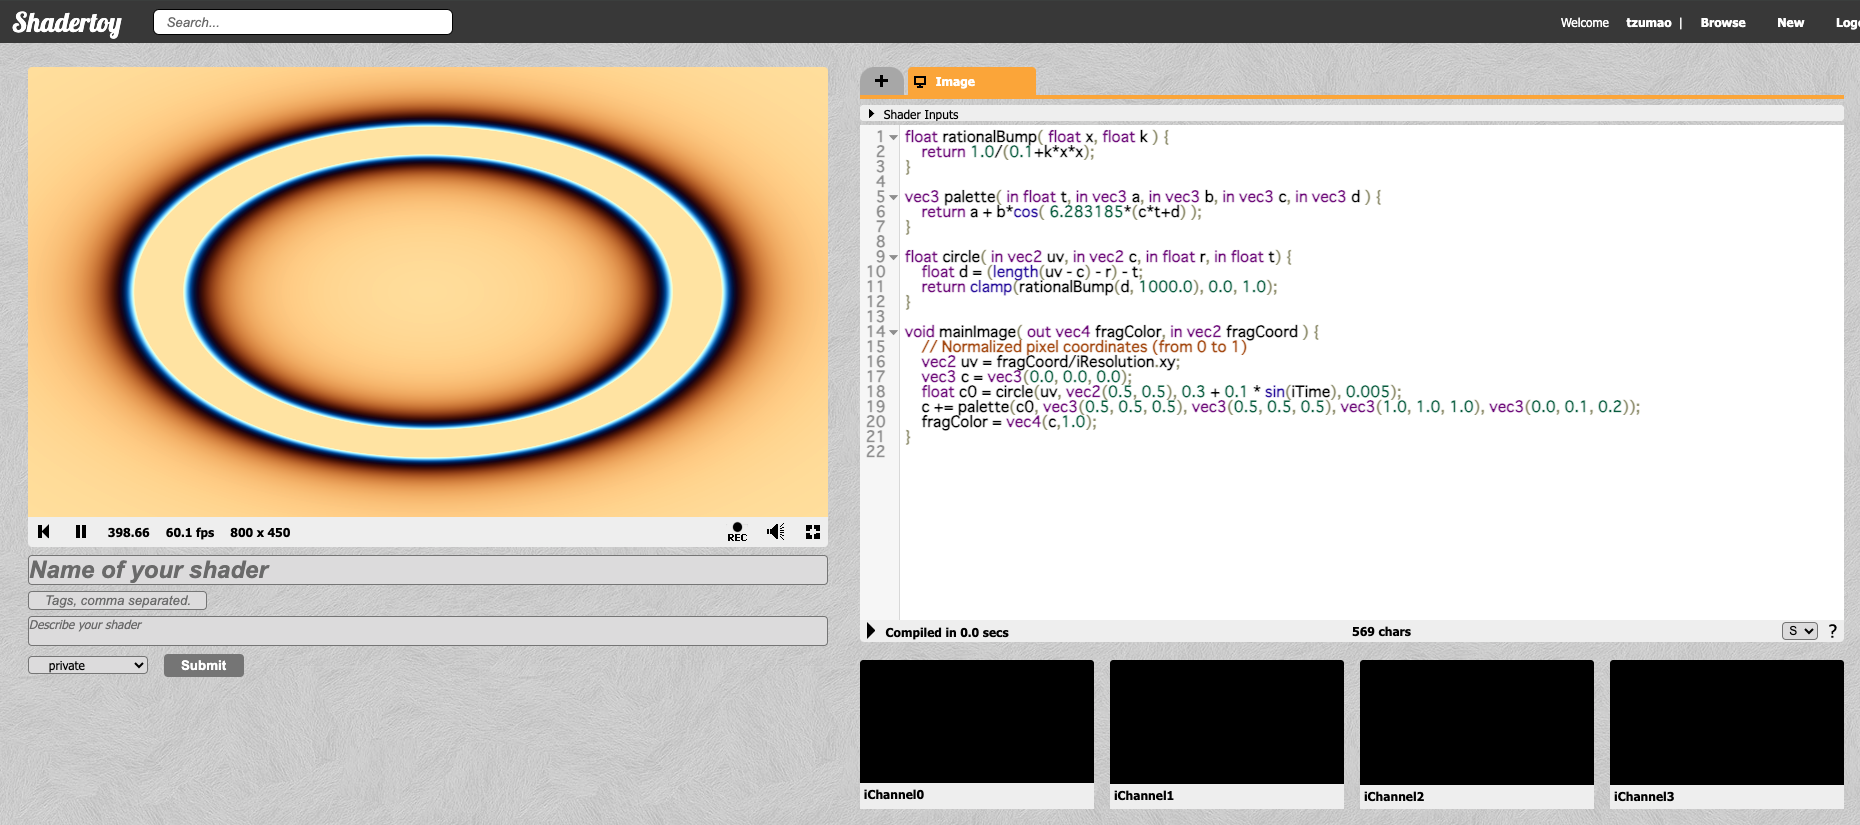
\includegraphics[width=0.80\linewidth]{imgs/circle_shader.png}
    \caption{A random shader I made on Shadertoy.}
    \label{fig:teaser}
\end{figure}

In this last assignment/final project, we will explore on producing some animations by writing code.
Instead of balboa, we will implement the animation in a very cool online service called \href{shadertoy.com}{Shadertoy}. In Shadertoy, all you have access to are a bunch of fragment shaders that draw to a quad. It is however a surprisingly powerful programming model that can be used to produce a wide variety of beautiful animations.

Before starting, take a look at the shaders other people wrote by clicking \emph{Browse} at the top-right of the shadertoy site. Note that these are all open source, so you can try to read their code (some of them are really short!). Here are a few ones I like (in no particular order):
\begin{itemize}
	\item \href{https://www.shadertoy.com/view/Ms2SD1}{Seascape} by TDM. 
	\item \href{https://www.shadertoy.com/view/ld3Gz2}{Snail} by Inigo Quilez.
	\item \href{https://www.shadertoy.com/view/lfscD7}{Hex Glitch} by igneus.
	\item \href{https://www.shadertoy.com/view/ddcGW8}{For the neon style enjoyers} by mrange.
	\item \href{https://www.shadertoy.com/view/4s23RW}{Glass crash} by Dave.
 	\item \href{https://www.shadertoy.com/view/XsBXWt}{Fractal land} by Kali.
 	\item \href{https://www.shadertoy.com/view/4ttSWf}{Rainforest} by Inigo Quilez.
 	\item \href{https://www.shadertoy.com/view/MfjyWK}{Starry Planes} by mrange.
	\item \href{https://www.shadertoy.com/view/ssjyWc}{Lover 2} by Fabrice Neyret.
\end{itemize}
Browse around and look at what other people created. Think about whether you can create the same.

To get started with shader art programming, here are two good Youtube videos by kishimisu. The first one introduces 2D shaders, and the second one introduces 3D shaders using raymarching.
\begin{itemize}
	\item \href{https://www.youtube.com/watch?v=f4s1h2YETNY}{An introduction to Shader Art Coding}
	\item \href{https://www.youtube.com/watch?v=khblXafu7iA}{An introduction to Raymarching}
\end{itemize}

For the project, submit a shadertoy link (\emph{please set the shadertoy project to UNLISTED, so that we do not spam the shadertoy browsing page}, you can set it back to public after the class ends) and a report documenting your journey: what have you tried, how did you reach your final art, etc. You will be graded by both technical sophistication and artistic values: you can have something that is technically cool but artistically uninspiring, or you can have something that is artistically interesting, but does not have that much technical content.
Your shader should be an animation, ideally with dynamic scenes instead of just panning cameras.

Below are some other resources that you can read/watch.

\paragraph{Storing and reading data across frames.} Sometimes you may want to store information from your fragment shaders and read from others. You will do it by writing to a texture using an extra fragment shader, then reading it back in another shader. See \href{https://www.shadertoy.com/view/tdGBDG}{this shadertoy tutorial} for how to achieve that.

\paragraph{Live coding sessions.} You can find some more coding sessions of how experts come up with their shaders on the internet. The Youtube channel The Art of Code also has some great content.
\begin{itemize}
	\item \href{https://www.youtube.com/watch?v=LLZPnh_LK8c}{Shader Coding: Over the Moon - Part 1}
	\item \href{https://www.youtube.com/watch?v=XaiYKkxvrFM}{Shader Coding: Over the Moon - Part 2}
	\item \href{https://www.youtube.com/watch?v=3CycKKJiwis}{LiveCoding - The Universe Within - Part 1}
	\item \href{https://www.youtube.com/watch?v=KGJUl8Teipk}{LiveCoding - The Universe Within - Part 2}
\end{itemize}

I also recommend the videos of Inigo Quilez, here are a few of them:
\begin{itemize}
	\item \href{https://www.youtube.com/watch?v=Cfe5UQ-1L9Q}{LIVE Coding "Happy Jumping"}
	\item \href{https://www.youtube.com/watch?v=sl9x19EnKng}{Live Coding "Sphere Gears" - Part 1}
	\item \href{https://www.youtube.com/watch?v=bdICU2uvOdU}{Live Coding "Sphere Gears" - Part 2}
	\item \href{https://www.youtube.com/watch?v=BFld4EBO2RE}{Painting a Landscape with Maths}
\end{itemize}

\paragraph{Particle systems.} An easy way to get cool animation is to use something call particle systems, where you represent a list of particles with individual positions, velocities, and other states. The particles can influence each other to create collective behaviors. Here are a few example shadertoys that implement a particle system:
\begin{itemize}
	\item \href{https://www.shadertoy.com/view/McXXzH}{Interactive particles} by berelium.
	\item \href{https://www.shadertoy.com/view/Xl2SRR}{Firework Show} by yibojiang.
	\item \href{https://www.shadertoy.com/view/4tKBDc}{Thermal particles} by wyatt.
	\item \href{https://www.shadertoy.com/view/WdSfzD}{Underwater Boids} by michael0804.
\end{itemize}

\paragraph{Mass spring systems.} Mass spring systems are another kind of cool way to implement physics. Instead of a collection of particles, we build a graph of vertices and create forces to push and pull vertices that have an edge between them. Below are some cool shadertoys that implement mass spring systems
\begin{itemize}
	\item \href{https://www.shadertoy.com/view/4fc3zf}{SpiderWeb} by middle.
	\item \href{https://www.shadertoy.com/view/llyBDW}{Lazy Cloth} by 834144373.
\end{itemize}

\paragraph{Fluid dynamics.} Fluids are another type of physical system that is relatively easy to implement (while the math is more involved), but can have very cool effects. A starter on this topic is Jos Stam's \href{http://graphics.cs.cmu.edu/nsp/course/15-464/Fall09/papers/StamFluidforGames.pdf}{Real-Time Fluid Dynamics for Games}. \href{https://www.shadertoy.com/playlist/X3dXR8}{This playlist} contains some cool shadertoys on fluid dynamics. Correct fluid simulation is subtle and I do not guarantee the correctness of those shaders, but one good thing about art is that it does not have to be correct!

\paragraph{Rigid body simulation.} Rigid body simulation is much harder in 3D than 2D. If you want to do this I recommend starting from 2D.
\begin{itemize}
	\item \href{https://www.shadertoy.com/view/MljSz1}{pool game physics} by archee.
	\item \href{https://www.shadertoy.com/view/NtlGz7}{2D Physics (balls)} by TDM.
	\item \href{https://www.shadertoy.com/view/MdXBD8}{physics engine} by archee.
\end{itemize}

Finally, \href{https://shadertoyunofficial.wordpress.com/}{Shadertoy Unofficial} is a cool blog documenting some cool shadertoy tricks.

\end{document}